\section{Selecting and training a network machine learning model}
\label{sec:ch2:select}

You've got your data loaded and pre-processed. Now comes the fun part: modeling your data. To do this, you first want to figure out the generative process that made it: what probabilistic model should you assume?

Next, you want to use that probabilistic model to create a reasonable representation for your data, often by moving from network space, with nodes and edges, to Euclidean space, with points on a coordinate axis.

Finally, you want to implement some downstream analysis method which helps answer whatever question you set out to answer.

\subsection{Generating new representations from your data}

As we briefly mentioned in Section \ref{sec:ch1:whatis}, a major problem with learning from network data is that networks in their rawest form are not tabular datasets. If you want to apply any of the breadth of knowledge acquired in general machine learning (which is typically designed for tabular datasets), you need to adapt your network to be compatible with tabular approaches, or adapt your general machine learning architecture for network layouts, such as adjacency matrices, which properly convey the dependences in network data. This is called \emph{representation learning}, and even neural networks typically do this under the hood with architectures like autoencoders.

Let's use a representation learning technique called a spectral embedding, which you will learn about in Chapter \ref{sec:ch6}. This technique will pop up many times, whether you are studying one network, pairs of networks, or multiple networks. Let's use it to embed our connectome:

\begin{lstlisting}[style=python]
from graspologic.embed import AdjacencySpectralEmbed

embedding = AdjacencySpectralEmbed().fit_transform(A_xfm)
\end{lstlisting}

An \emph{embedding} takes the adjacency matrix, which is a matrix representation of the entire network, and turns it into a tabular array. Each row is called an \emph{estimated latent position} for a given node, and each column is called an \emph{estimated latent dimension} of the network. If there are $n$ nodes, there are $n$ rows of the spectral embedding, and if there are $d$ estimated latent dimensions of the network, there are $d$ columns. The spectral embedding has taken the $n \times n$ adjacency matrix, which we can't use traditional machine learning algorithms on, and transformed it into a $n \times d$ tabular array, which we can use machine learning algorithms on. We'll visualize this embedding using a \emph{pairs plot}, which is a scatter plot where each node is a single point in the plot, and the x and y axes are different \emph{pairs} of latent dimensions for that particular node:

\begin{lstlisting}[style=python]
from graspologic.plot import pairplot

_ = pairplot(embedding, title="Spectral Embedding for connectome")
\end{lstlisting}
This pairs plot is shown in Figure \ref{fig:ch2:pairplots}(A).

As it turns out, this particular representation of the adjacency matrix through the spectral embedding can be tied into a statistical model if you make some assumptions. In particular, those of the stochastic block model described in Section \ref{sec:ch5:sbm}. The stochastic block model says that each node is a member of a subgroup, called a \emph{community}, and its connectivity to other nodes in the network is dictated by which community it is a member of, and which community the other node is a member of. This sounds a \emph{lot} like the question that your colleague wanted you to approach, since it gives a way to take the nodes of the network and form ``functionally similar'' subgroups from them. 

\subsection{Using your representations to learn new features from the network}

Now that we have a tabular representation of the data, we can attempt to use the intuition and assumptions of the stochastic block model to cluster our nodes. Let's see what happens when we apply \texttt{KMeans} to our data:
\begin{lstlisting}[style=python]
from sklearn.cluster import KMeans

labels = KMeans(n_clusters=2).fit_predict(embedding)
_ = pairplot(embedding, labels=labels, legend_name="Predicter Clusters", 
                 title="KMeans clustering")
\end{lstlisting}

The results of this pairs plot are shown in Figure \ref{fig:ch2:pairplots}(B).
\begin{figure}
    \centering
    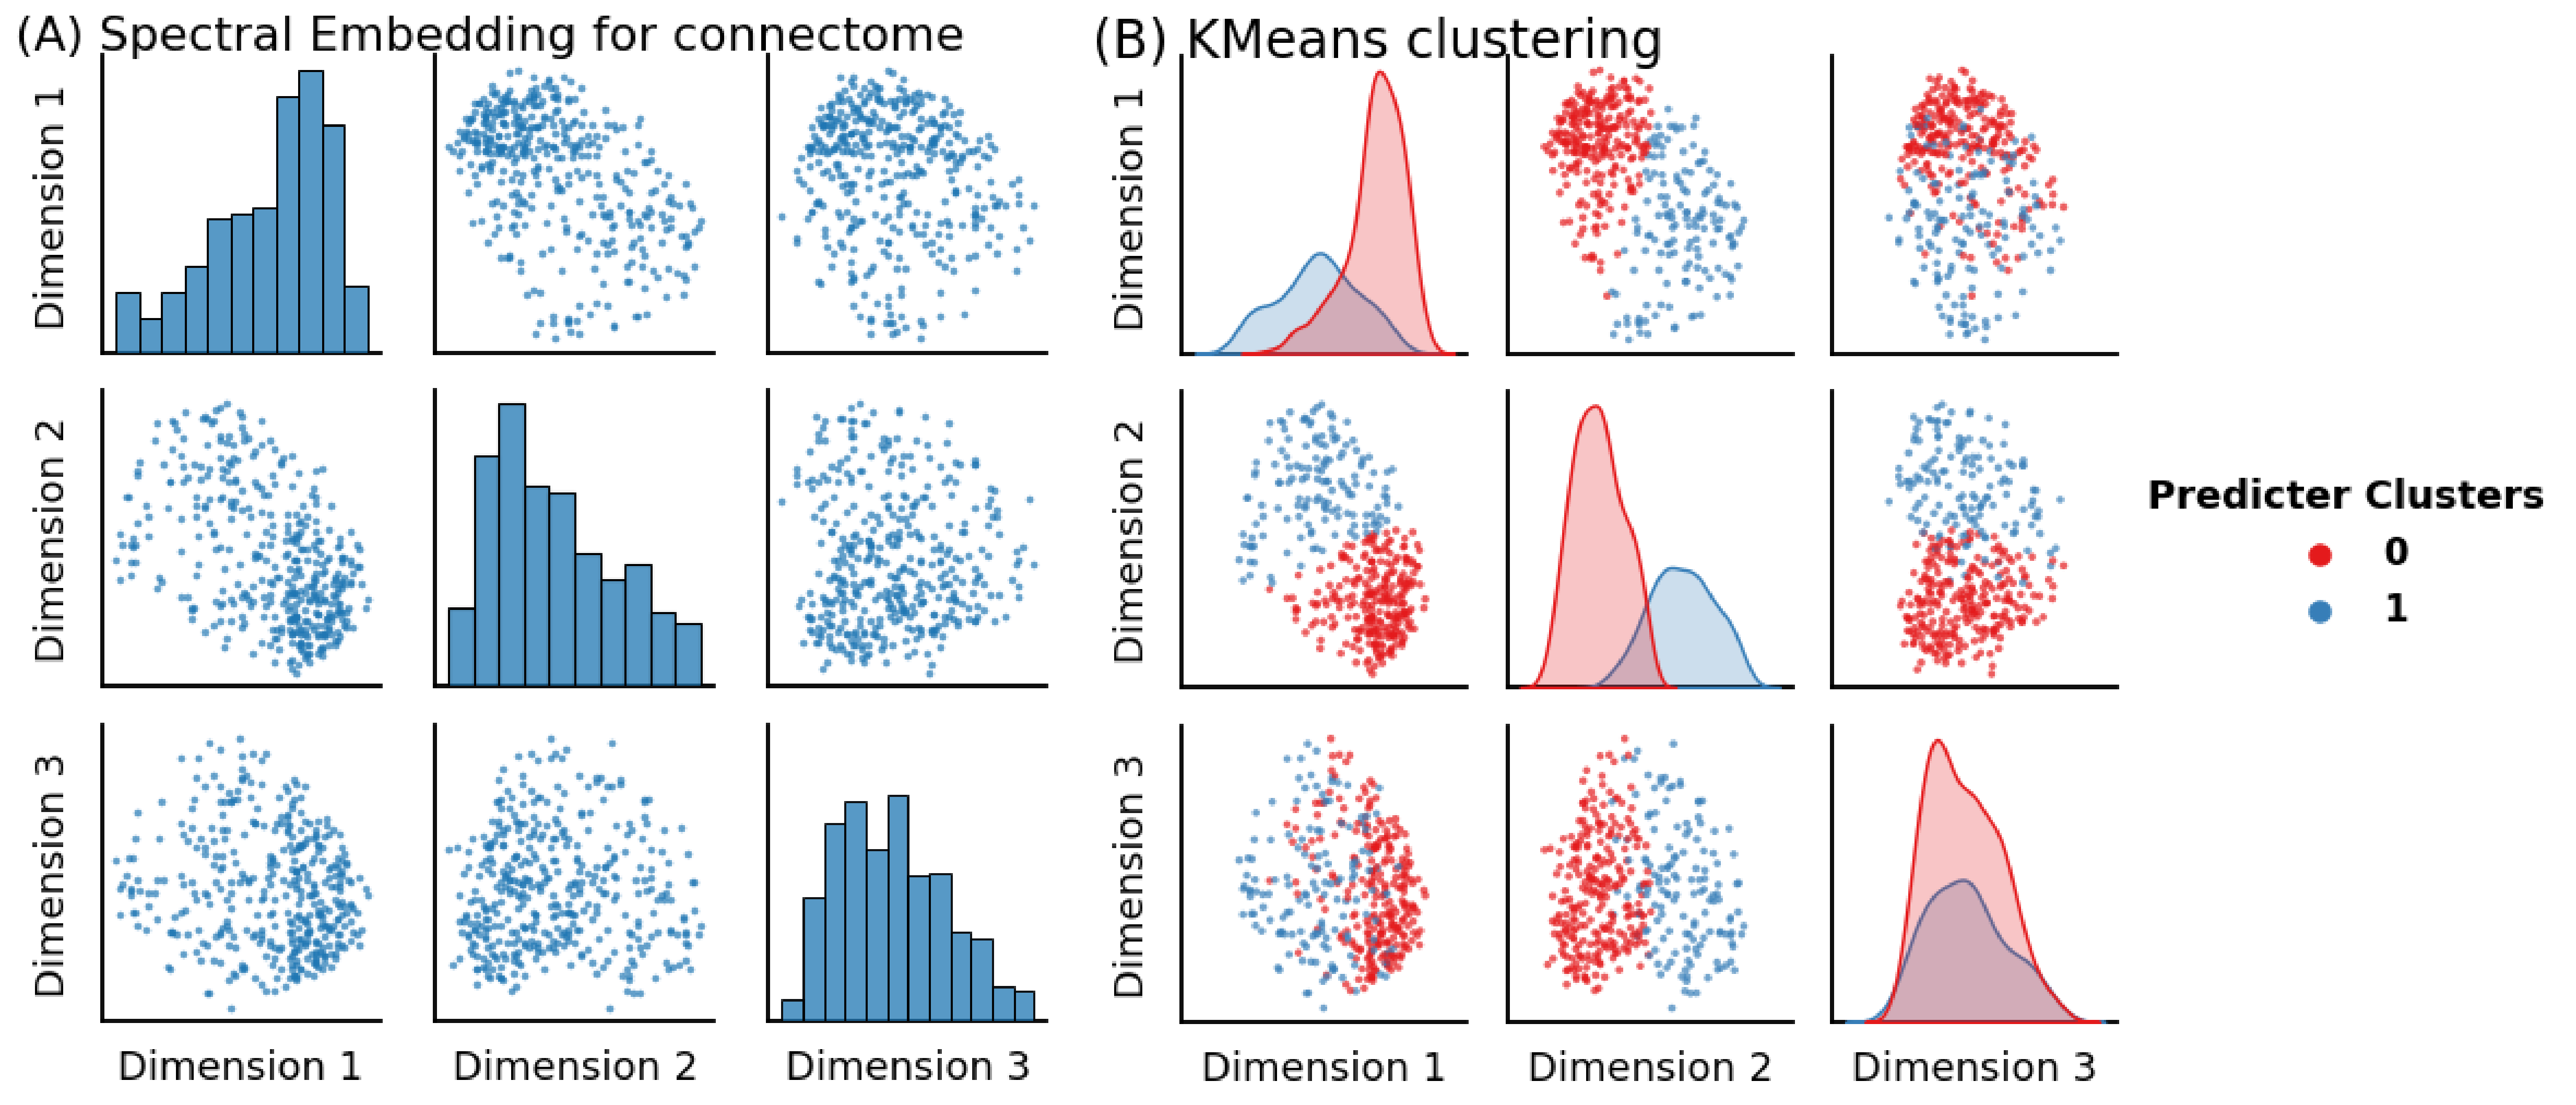
\includegraphics[width=\linewidth]{foundations/ch2/Images/pairplots.png}
    \caption[The pairs plot for embedded connectomes]{\textbf{(A)} The  pairs plot for the estimated latent dimensions. \textbf{(B)} The  pairs plot with predicted communities of nodes via \texttt{KMeans} with $2$ clusters.}
    \label{fig:ch2:pairplots}
\end{figure}
So, it looks like the $k$-means was able to learn $2$ clusters from our dataset. These clusters are indicated by the ``blobs'' of points that are red or blue, respectively.

If you're careful, you'll notice we did something a little weird here. Why did we choose $2$? Why not $5$? Why not $8$? We chose $2$ somewhat arbitrarily. In general, when you don't know what to expect from your data (we didn't know what to expect here, other than that we wanted a modestly sized way to group the nodes up), it's a good idea to use quantitative means to make these determinations for you. 

With \texttt{KMeans}, we can use something called the silhouette score to do this for us. You choose the optimal number of clusters as the clustering with the highest silhouette score (This is covered in Section \ref{sec:ch7:comm_detect} when you learn about community detection). \texttt{graspologic} makes this process pretty straightforward with a \texttt{KMeansCluster} class, which uses the silhouette score under the hood:

\begin{lstlisting}[style=python]
from graspologic.cluster import KMeansCluster

labels = KMeansCluster(max_clusters=10).fit_predict(embedding)
_ = pairplot(embedding, labels=labels, title="KMeans clustering, automatic selection", 
                 legend_name="Predicted Clusters")
\end{lstlisting}
Unlike the previous approach, it looks like with silhouette score selection, we ended up with $5$ clusters being optimal, not $2$. The pairs plot for the embedded data with the new labels are in Figure \ref{fig:ch2:pairplots_impute}(A). Note that you might get a different number of estimated clusters than we did, because there is some randomness in the unsupervised learning procedure that we used here.

So, what about other possible approaches? Unless you are pretty confident that the clusters you are looking for have ``blobs'' that are totally spherically symmetric (basically, they look like ``balls'' in the dataset), $k$-means can be a pretty bad idea. Another strategy called the gaussian mixture model, or \texttt{GMM}, handles this a bit more elegantly, allowing your cluster blobs to be pretty much any ellipse-like shape. We can use \texttt{GMM} and automatically select the number of clusters using the Bayesian Information Criterion, or BIC, with \texttt{AutoGMMCluster}:
\begin{lstlisting}[style=python]
from graspologic.cluster import AutoGMMCluster

labels = AutoGMMCluster(max_components=10).fit_predict(embedding)
_ = pairplot(embedding, labels=labels, title="AutoGMM Clustering", 
                  legend_name="Predicted Clusters")
\end{lstlisting}
The pairs plot for the embedded data with the labels determined by \texttt{GMM} in Figure \ref{fig:ch2:pairplots_impute}(B). It looks like GMM actually found $4$ clusters to be a bit more optimal than $3$ clusters. 

\begin{figure}
    \centering
    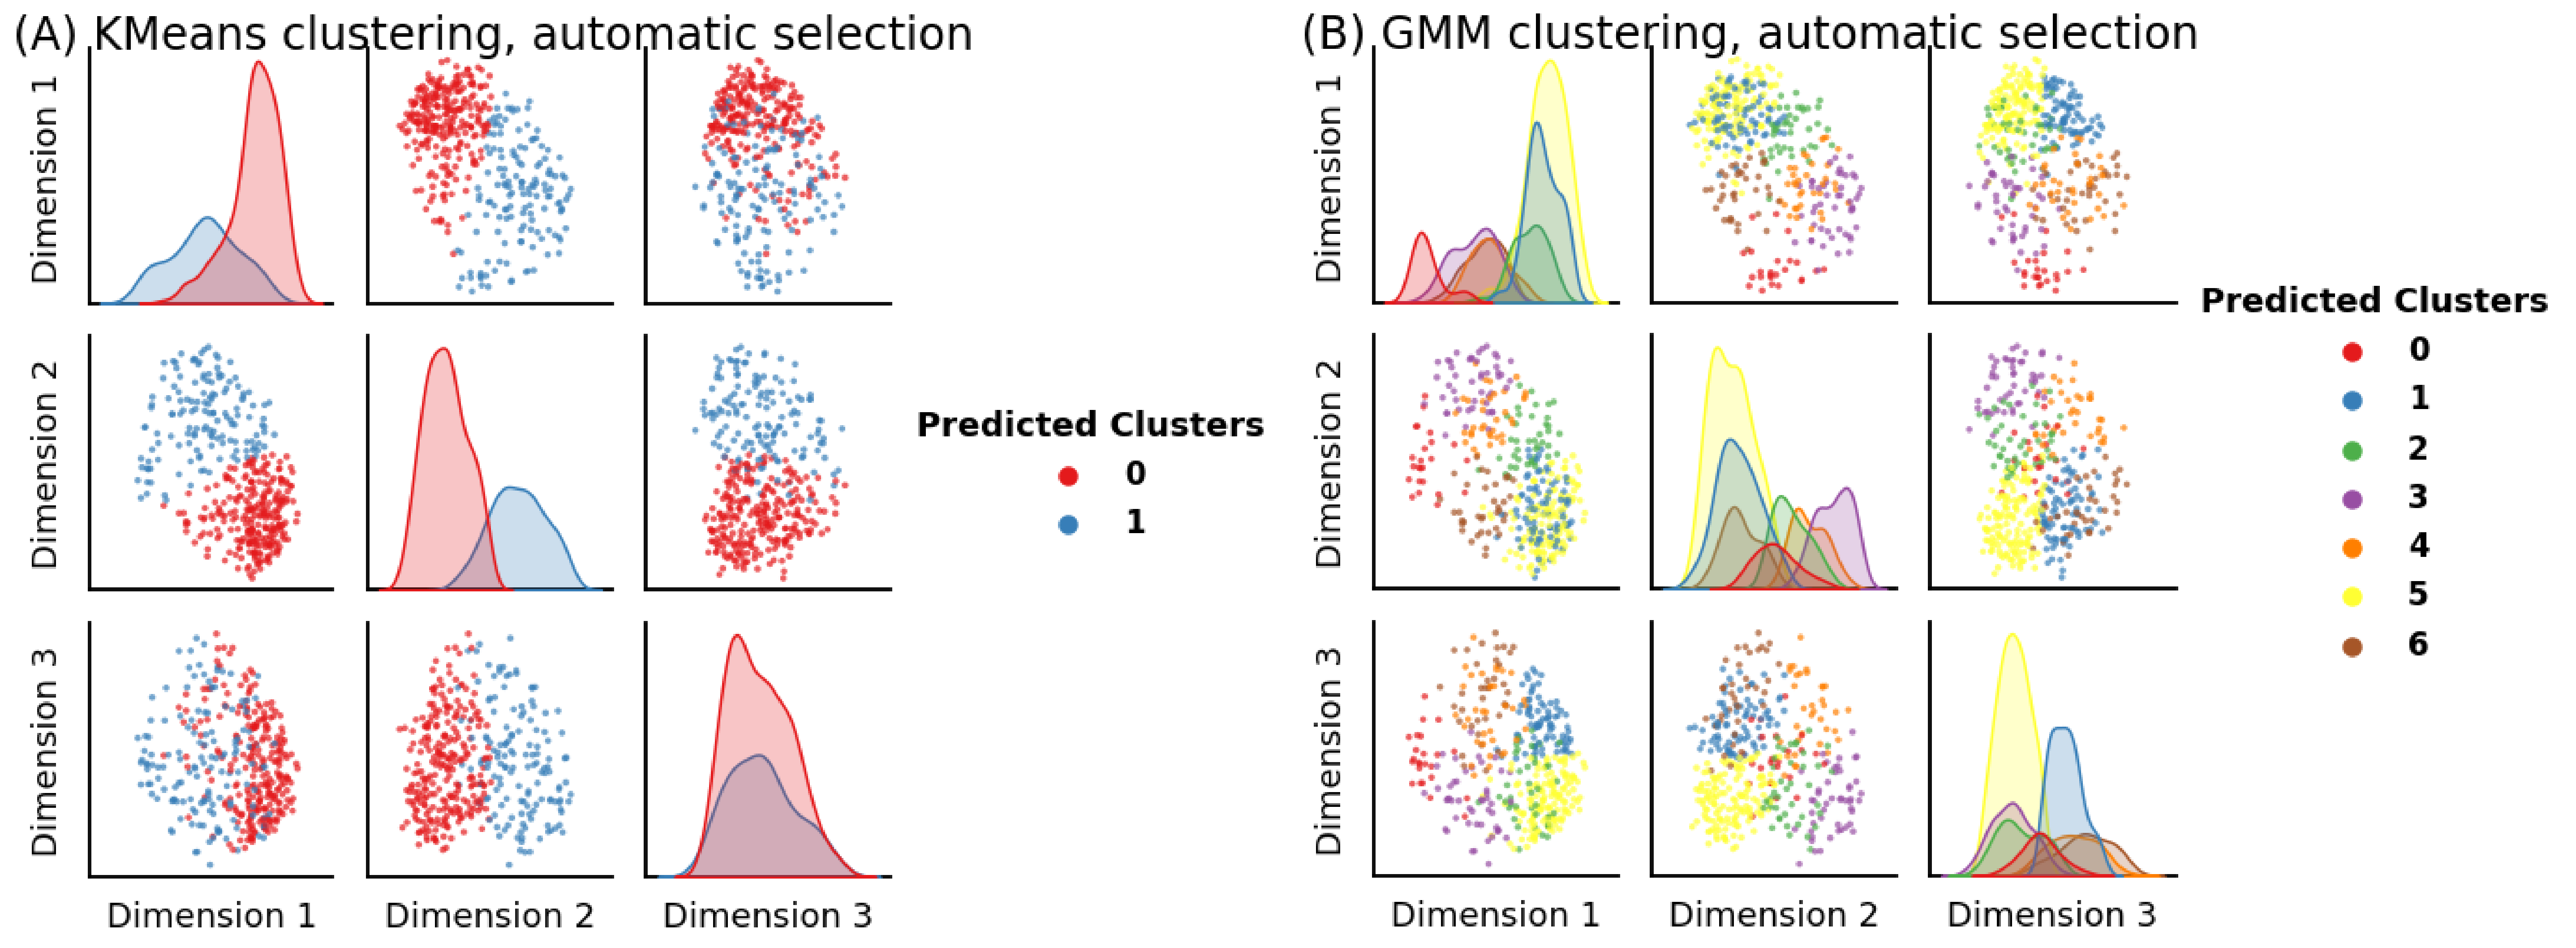
\includegraphics[width=\linewidth]{foundations/ch2/Images/pairplots_impute.png}
    \caption[Comparison of labels estimated by $k$-means and GMM]{\textbf{(A)} the pairs plot for the embedded data, with node communities estimated by \texttt{KMeans}. \textbf{(B)} the pairs plot for the embedded data, with node communities estimated by \texttt{GMM}.}
    \label{fig:ch2:pairplots_impute}
\end{figure}

\newpage